\subsubsection{FRI}\label{section: starky-fri}

\begin{figure}[!htp]
    \centering
    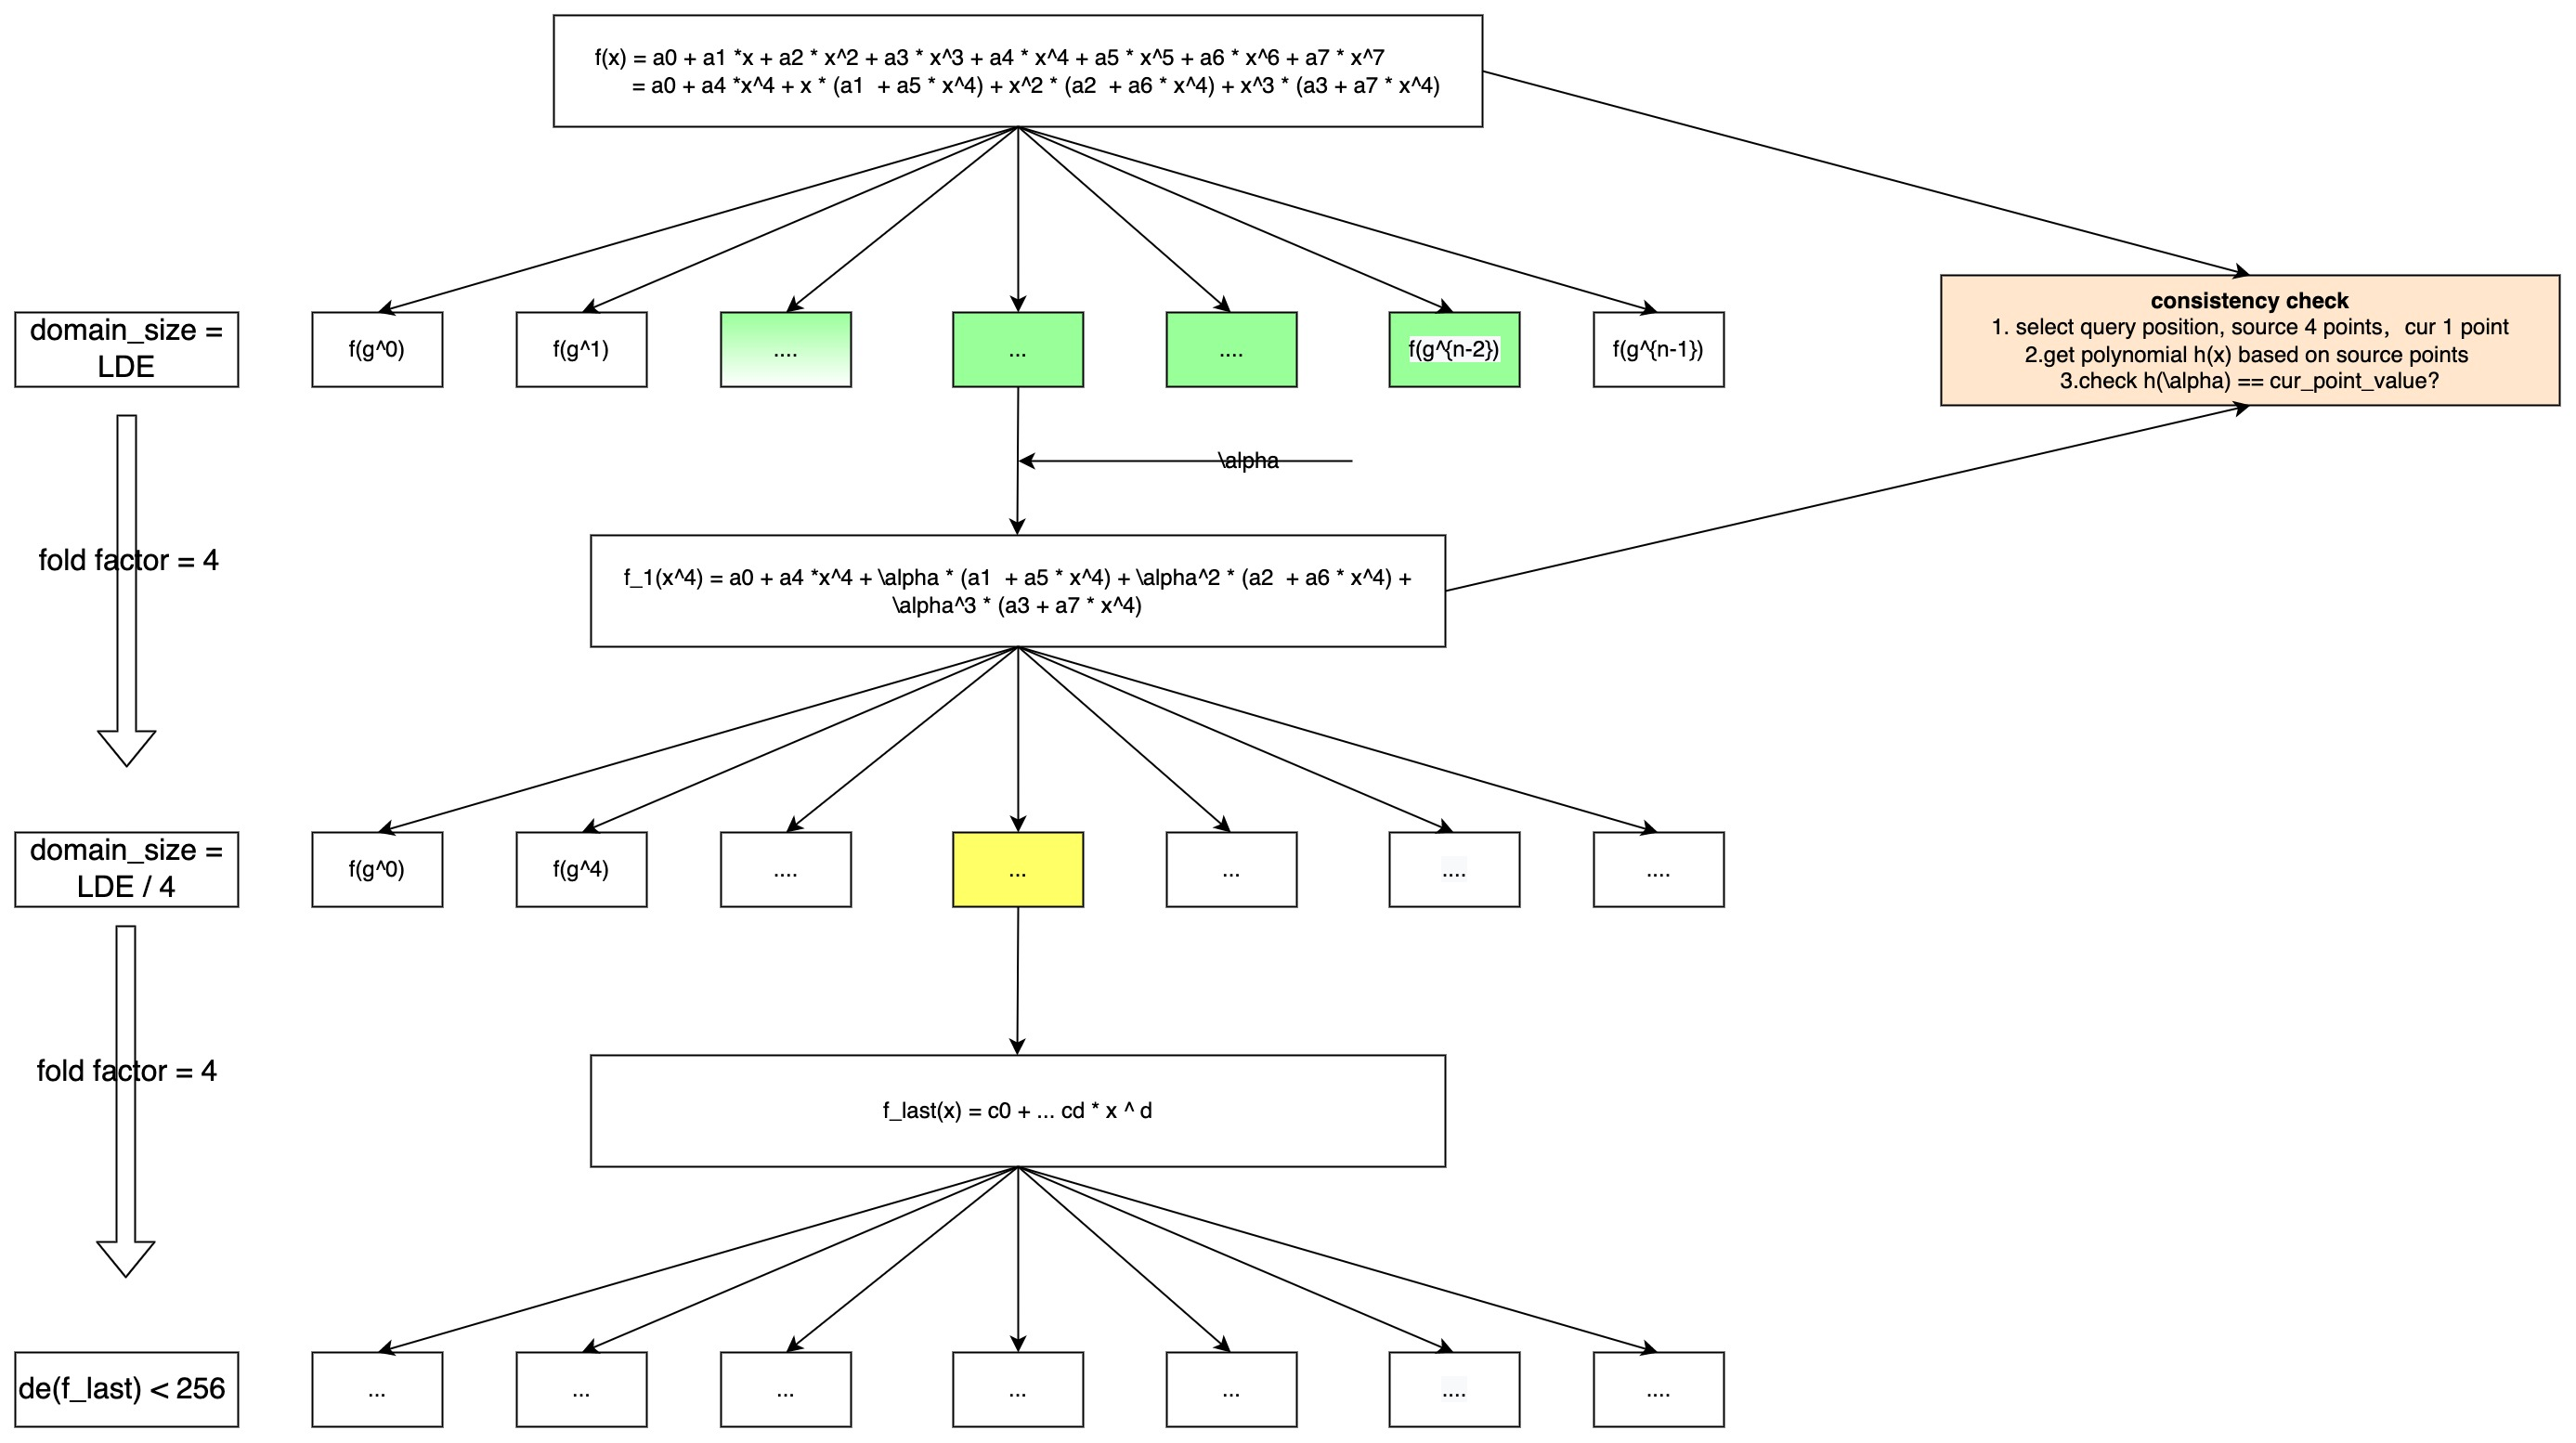
\includegraphics[width=0.8\textwidth]{fri.jpg}
    \caption{FRI protocol}
    \label{fig: FRI}
\end{figure}

FRI is a protocol that proves a committed polynomial having a bounded degree. Ola uses Deep-FRI for its polynomial commitment scheme. \figref{fig: FRI} simply expresses the calculation process of FRI, anyone can read DEEP-FRI \cite{cryptoeprint:2019/336} for more details.
